\chapter{Literature Review}

% Split into two main sections: fields and techniques; mathematical background

% Lit review structure
% ML intro as subset of AI
% NNs
% Note on AI winter
% SVMs
% DL emerges - note on previous aspersions on this
% Image recognition
% Expansion to other domains and architectures
% Acceleration, hype (media coverage, publicity etc, large industrial use Tesla etc)
% Emphasis on loss functions and explanation
% History of Random Projections
% Narrow down to flip probability specifically
% Mention use in logistic regression and bounds on error for linear classification

\section*{Fields and Techniques}

%\begin{SCfigure}
\begin{wrapfigure}{r}{0.5\textwidth}
    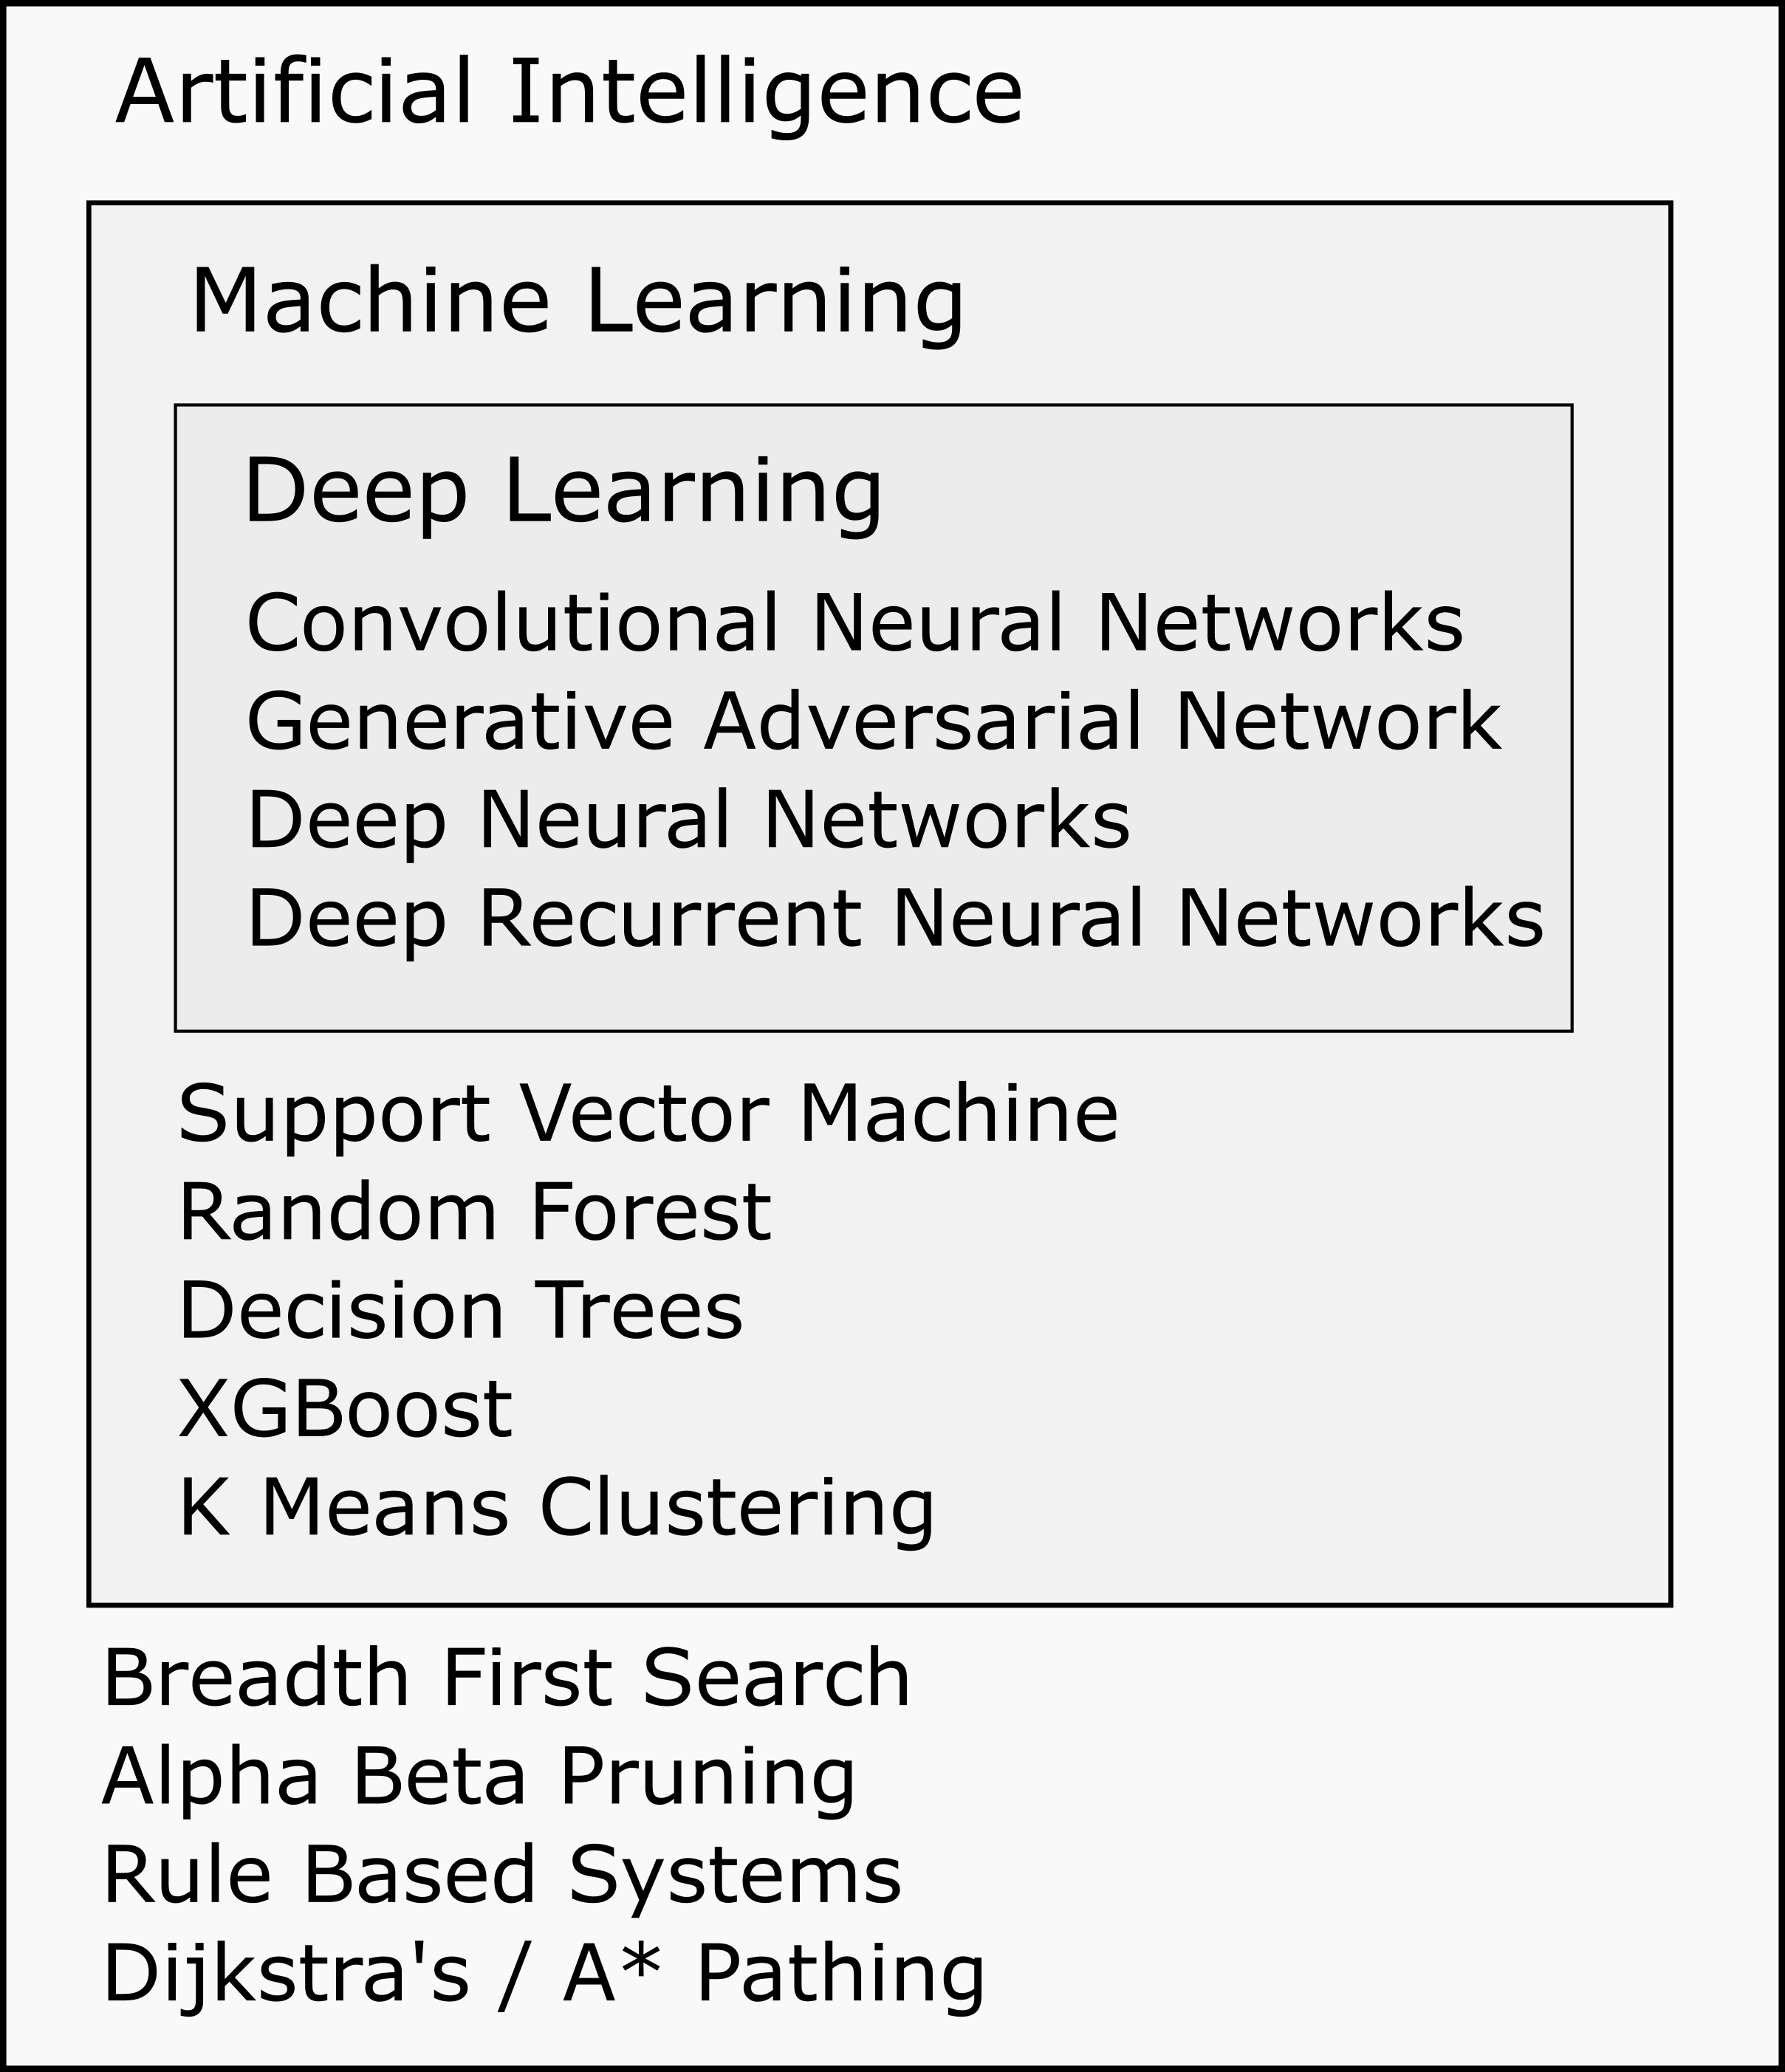
\includegraphics[width=80mm]{figs/ai_ml_dl.png}
    \caption{The fields of \gls{ai}, \gls{ml} and \gls{nn}, with examples of techniques in each.}
    \label{fig:ai_ml_dl} 
\end{wrapfigure}

%\end{SCfigure}
Figure \ref{fig:ai_ml_dl} shows the relationship between \gls{ai}, \gls{ml} and \gls{dl}. \gls{ai} concerns the broad field of using technology to mimic human behaviour. \gls{ml} additionally involves training algorithms to find rules automatically based on training data, which can involve techniques usually situated within statistics, such as linear or logistic regression. \gls{dl} takes this a step further, concern the use of multi-layered \gls{nn}s trained on a large pool of training data to perform even more complex tasks, such as image segmentation or video captioning. The roots of \gls{ai} goes to the 1950s, with one particular event, the Dartmouth Summer Research Project, gaining particular retrospective notoriety for proposing to making significant advances in the field in a '2 month, 10 man study'  \cite{dartmouth_summer}.

\section{Machine Learning}
% name drop kernel trick

\gls{ml} is an interdisciplinary field at the intersection of mathematics, computer science and statistics and itself is often considered as a sub-field of the broad area of study that is  \gls{ai}. \gls{ml} deals with the challenge of "learning" from data without manual human input. In contrast to many statistical techniques, \gls{ml} is especially suited to scenarios where predictive accuracy is paramount, training examples are both numerous and high dimensional, and inferential understanding is not critical [ZAMBINGO]. \gls{ml} gathered a lot of momentum in the 1990s, with the term 'data mining' often used as a pseudonym. Traditional techniques in the field of \gls{ml} include decision trees,  \gls{svm}s, K-means clustering, Naive Bayes and  \gls{flda}.  \bigskip

% probably delete this line 
Examples of classic data sets in \gls{ml} refer to unsupervised classification of data points into flower species, predicting diabetes risk based on a small subset of predictors, predicting whether a mine is present based on hundreds of frequency reflection variable and other challenges \cite{uci_ml_data}. Practical milestones include the use of Yan Le Cun's 'LeNet' architecture in the late 1990s to perform accurate handwriting recognition. At one stage, this algorithm (a \gls{cnn}) was responsible for the majority of automated cheque processing in the United States [ZAMBINGO].  \bigskip

The key idea is that the algorithm automatically finds and determines a set of rules to effectively label the input data based on some learning process that seeks to find the optimal set of model parameters. This avoids, for example, algorithms that are highly task specific (such as searching algorithms or algorithms specifically designed to find the optimal move given a particular rule set). \bigskip

\section{Neural Networks} 

\gls{nn}s (in this work, networks, \gls{ann}s and 'nets' all refer to \gls{nn}s) started with the perceptron which then evolved onto the \gls{mlp}. Later, multi-layer \gls{ffnn}s were used, and the the architecture diversified into the \gls{cnn}s with the use of local receptive fields. A timeline of developments and architectures is present in figures \ref{fig:timeline_new_nn} and \ref{fig:timeline_old_nn}. \bigskip

\begin{figure}
    \centering
    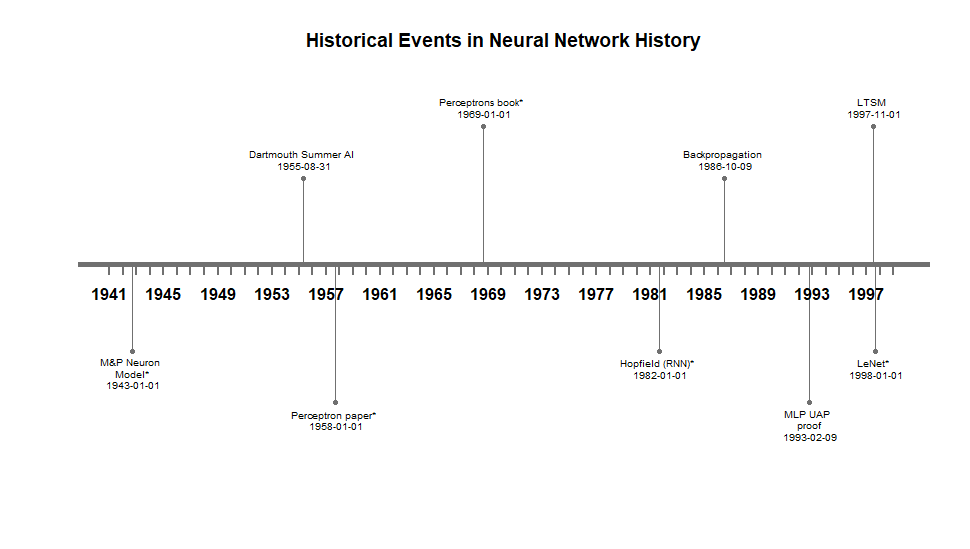
\includegraphics[width=160mm,scale=1.5]{figs/timeline_old_nn.png}
    \caption{A selection of events in early neural network history}
    \label{fig:timeline_old_nn}
\end{figure}

\begin{figure}
    \centering
    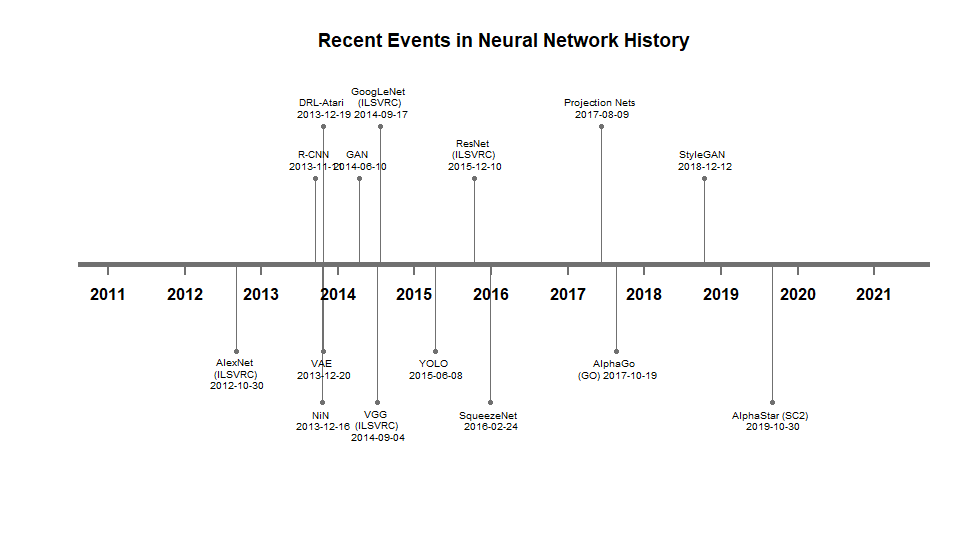
\includegraphics[width=160mm,scale=1.5]{figs/timeline_new_nn.png}
    \caption{A selection of events in modern neural network history}
    \label{fig:timeline_new_nn}
\end{figure}

Figures \ref{fig:timeline_old_nn} and \ref{fig:timeline_new_nn} show a small selection of key historic and recent events. Major recent events include progress made in \gls{drl}, such as teaching a network to effectively play a variety of Atari games without any manual intervention \cite{drl_atari}. Generative networks progressed, with the development of \gls{vae}s, which could generate examples from complex distributions and were then surpassed by the development of \gls{gan}s for the generation of highly realistic examples \cite{gan}. AlphaStar  \cite{alpha_star} and AlphaGo \cite{alpha_go} gained a lot of attention \cite{press_alpha_go} \cite{press_alpha_star} for beating top human players in the board game Go and the video game StarCraft II. Both games are notably complex with the first having an extremely large state space (having around 300 possible moves on average, versus an average of \cite{moves_chess_go}) and the second having a complex continuous real time state space, often requiring  around 400 \gls{apm} \cite{sc_apm} for top human players. Style\gls{gan}s were notable for effective image style transfer, which was also picked up in the media \cite{press_stylegan} \footnote{An interactive example of this can be found here \url{ZAMBINGO}}.

In terms of \gls{cnn}s, kicked off a flurry in research activity in \gls{dl}, as it was the first \gls{dnn} to win the \gls{ilsvrc}, in 2012 \cite{alex_net}. \gls{r-cnn}s were notable for classification of regions and \gls{semanticsegmentation} using \gls{cnn}s. 'GoogLeNet' introduce a more parallel architecture with the 'inception' module to achieve higher accuracies \cite{googlenet}. \gls{resnet}s broke new ground with it's extreme depth \cite{resnet} by surpassing 'human level recognition' \cite{resnet_human}. 'SqueezeNets' introduce high performing \gls{cnn}s with far fewer parameters and a smaller memory footprint \cite{squeeze_net}. 
\bigskip

A \gls{nn} can be interpreted many ways. For example, a common interpretation is that \gls{nn} act as function approximation machines, a view influence by the \gls{uap} theorem for \gls{mlp}s, which states that;

\begin{quote}
    A standard multilayer feedforward network with a locally bounded piecewise continuous activation function can approximate any, continuous function to any degree of accuracy if and only if the network's activation function is not a polynomial.\cite{uap_mlp}
\end{quote}

Another view of \gls{nn}s is as an extremely simply approximation of how the brain works. 

At it's simplest, it is a single \gls{neuron} comprising of a weighted sum of the input features, the addition of bias term and the application of an \gls{activationfunction} to provide an output for a given input instance $i$;

\begin{figure}
    \centering
    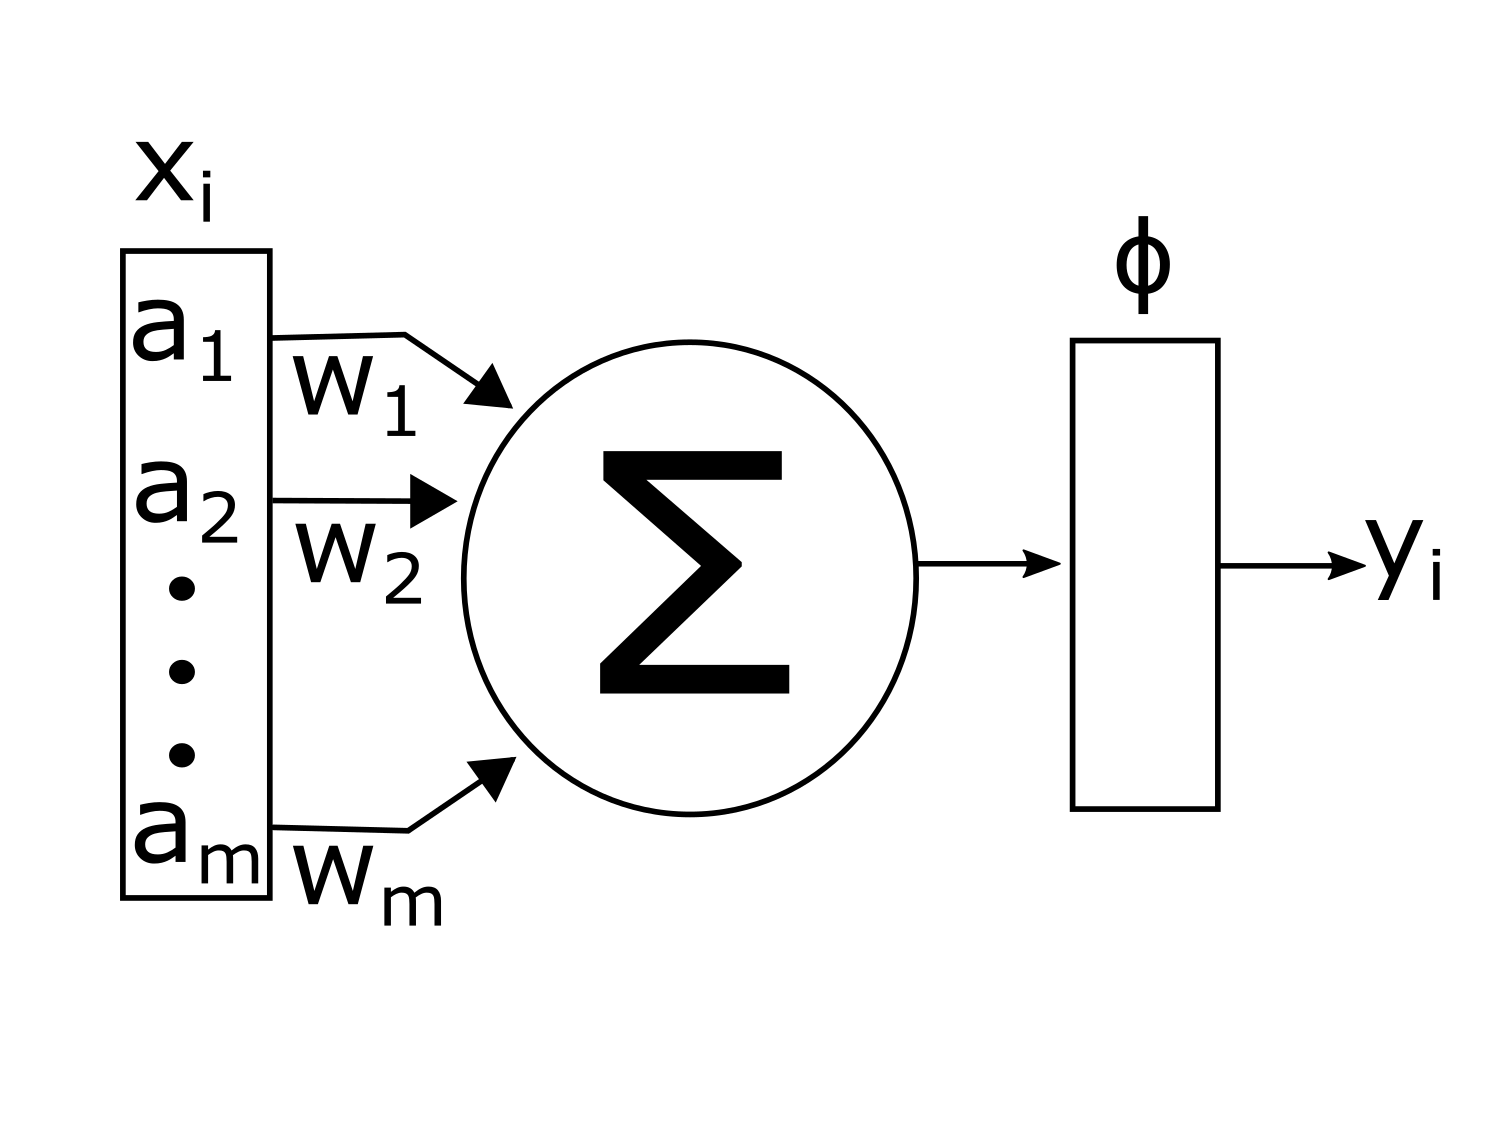
\includegraphics[width=100mm]{figs/nn_simple.png}
    \caption{The prediction process for a single point of data in a perceptron.}
    \label{fig:nn_simple}
\end{figure}

\begin{equation}
    y_i = \mathds{1} ((\sum_{j = 1}^m w_j + b_m) > 0)
    \label{eq:sgd_fp}
\end{equation}

This network is a \gls{linearclassifier}, which has a single \gls{layer} and uses the heaviside \gls{activationfunction} (figure \ref{fig:heavi_function}). 

\begin{wrapfigure}{l}{0.5\textwidth}
    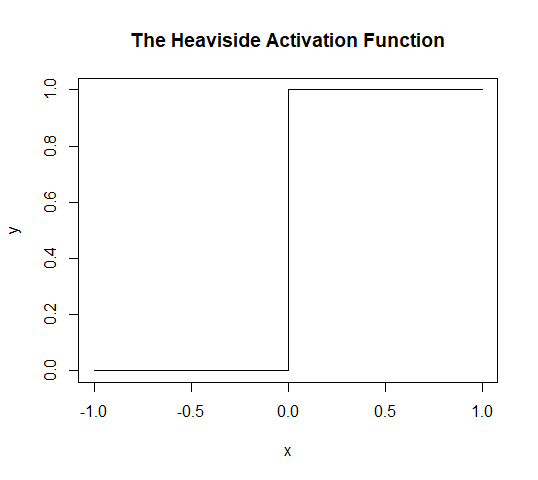
\includegraphics[scale=0.5]{figs/heavi.png}
    \caption{The Heaviside activation function.}
    \label{fig:heavi_function}
\end{wrapfigure}

Choosing an activation function when designing networks in modern times often comes down to using the 'tried and true' functions, or a lot of manual \gls{hyperparameter} tuning.

\gls{nn}s find their origins in the fields of psychology and electronic engineering, dating back to the days of linear adaptive filters in the \cite{nns_haykins}. This began perceptron model proposed by Rosenblatt \cite{perceptron_paper} as an extension of the McCulloch and Pitts model of the neuron \cite{logical_calculus} \bigskip

% REDO DIAGRAM IN GGPLOT2
\begin{figure}
    \centering
    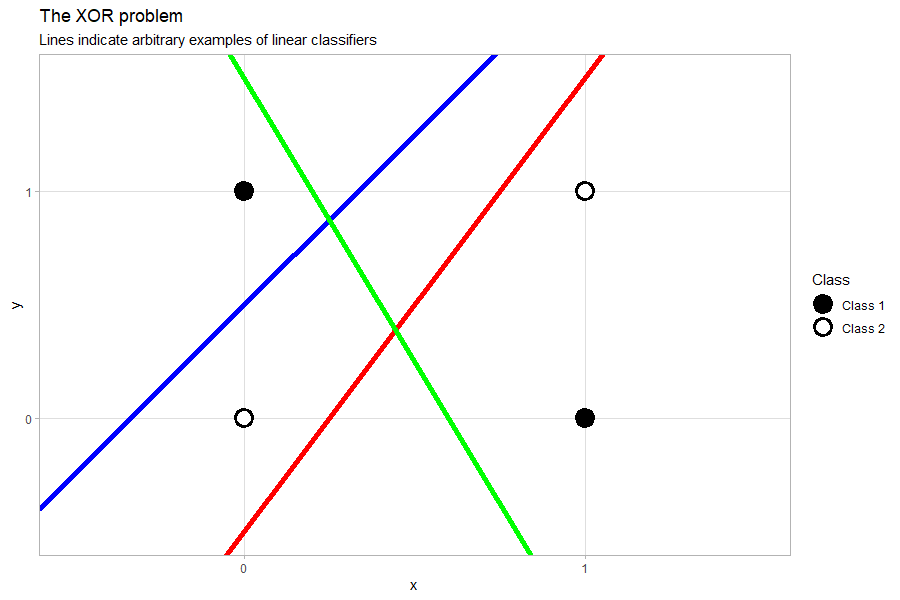
\includegraphics[width=120mm]{figs/xor_problem.png}
    \caption{An illustration of the \gls{xor} problem that a perceptron can not solve.}
    \label{fig:xor_problem}
\end{figure}

The \gls{xor} problem is the simplest possible example of data that is not \gls{linearlyseparable}. After the highly influential book,'Perceptrons' proved that the \gls{xor} problem (figure \ref{fig:xor_problem}) could not be solved with a single layer perceptron \cite{perceptrons_book}, interest in neural networks died off considerably - this is often referred to as the 'AI winter' \cite{ai_winter}. It has been speculated \cite{ai_winter} that this was in part because the idea that \gls{mlp}s could not solve the \gls{xor} problem gained traction, despite the authors acknowledging that it was likely that they could in their book [ZAMBINGO]. \bigskip

Eventually however, research with layered \gls{nn}s intensified and progress was made, not least in part because of advances in computational power;

\begin{quote}
...the IBM 704 computer that cost \$2 million in 1958, or \$20 million in today’s dollars, could perform 12,000 multiplies per second, which was blazingly fast at the time. The much less expensive Samsung Galaxy S6 phone, which can perform 34 billion operations per second, is more than a million times faster...\cite{unreasonable_dl}
\end{quote}

%todo insert xor figure

\bigskip
Coming out of the AI winter, \gls{nn}s were restricted to four or five layers (never past ten). There was a 'node budget' and a lot of manually configured architecture at the node level. The manually specified architecture of the network was critical to it's success [ZAMBINGO], for example in computer vision, where significant amounts of feature engineering was required. 

In 1997, Yan Le Cun developed the first neural network capable of high accuracy digit recognition which outperformed the previously popular \gls{svm} models. \bigskip

% feed forward neural network

% CNN

\section{Deep Learning}

Highly layered ("deep") \gls{nn}s lie at the heart of \gls{dl} and are in fact all extensions of the \gls{mlp}. Other deep algorithms do exist (such as 'deep trees' \cite{deep_forest}) although these are unable to handle complex image classification problems as well as other modern {dnn}s. \gls{dl} is seen as a highly effective strategy in a variety of \gls{ai} applications. As a model, they are far more complex than most statistical models, having millions of parameters \cite{unreasonable_dl}.  \bigskip
% AI winter mention and comeback - LeNet CNNs then cooling SVMs

For context \gls{nn}s had now significantly fallen out of favour [ZAMBINGO] and \gls{svm}s were rapidly gaining popularity [ZAMBINGO]. This trend continued until 2012, when the striking performance of AlexNet, a \gls{dcnn}, in the influential annual \gls{ilsvrc} created a lot of interest in \gls{dl}. The remarkable improvements in performance achieved showed the viability of \gls{dl} as an alternative to \gls{svm}s and other techniques, for \gls{imagerecognition}. This demonstration was enabled by several factors contributing to recent rapid developments in \gls{dl}: the availability of \gls{dl} tool-kits, such as Theano and Caffe (2007, 2013 - REF), and Keras, TensorFlow and PyTorch (2015, 2016 ZAMBINGO); advances in computational hardware and accessibility, including powerful purpose-built \gls{gpu}s (examples... mention google TPUs?), accessible to cloud compute (\gls{aws}, \gls{gcp}, Azure) and decreasing cost barriers (Google Collab, MatrixDS, note on costs e.g. declining storage costs); and access to large, curated data sets for training (large text corpuses, image repositories, [ZAMBINGO]) \bigskip

Now, \gls{nn}s can be incredibly deep, from 50-150 layers (depths used with \gls{resnet}s \cite{resnet}) and also quite wide (such as 

% insert summary table of models used in ILSVRC, number of parameters, hardware trained on, architecture, unique features and top 1/3/5 accuracy's

% when to capitalise fields?
While this was a major advancement for \gls{dl} in the problem domain of image classification, progress was being made in other domains; speech recognition, handwriting recognition, image segmentation, image captioning, generative models [ZAMBINGO] \bigskip % todo - finish list of progress in domains
 
\gls{dl} has evolved as a subset of \gls{ml} methods used for extracting complex semantics from data. \gls{dl} methods have achieved a wide variety of goals that would not otherwise be possible via traditional machine algorithms (such as realistic face generation \footnote{For an excellent example of this, see \url{https://www.thispersondoesnotexist.com/}, for realistic faces generated by StyleGANs})  \bigskip% todo - finish list of goals 

The success of  \gls{dl} has fuelled the development of a plethora of different  \gls{nn} architectures, including \gls{ltsm}s, \gls{rnn}s and \gls{gan}s [ZAMBINGO]. These are now widely used in a variety of applications, such as for text-to-speech, handwriting recognition and art generation (respectively). [ZAMBINGO]  \bigskip 

\section{Convolutional Neural Networks}

\gls{cnn}s were inspired by the 'Neocognitron' of the 1980s \cite{neocognitron} and were developed in earnest by in the 1990s, with early uses involving reading cheques \cite{lecun_cheques}. The primary purpose of \gls{cnn}s is \gls{imagerecognition}, although they are also used in time series forecasting (1D \gls{cnn}s) and can be used for 3D recognition, for example using sensors from the Microsoft Kinect (\cite{3d_conv}). \gls{cnn}s hinge on 'local receptive fields' (also known as sparse connectively), which means that each of the input layer neurons have a particular patch of the input data that they connect to. The input data (or function) undergoes a convolution, in that a filter (or kernel) is convolved (slid across) the data. Each successive neuron in a given layer \cite[Chapter~5]{good_fellow_2016}

%removed "generally"

\section{Applications}

Image classification is a subset of the broader area of computer vision, which includes such applications as face detection, object detection, image segmentation, feature detection

%The field of \gls{dl} is a relatively modern one, and recent developments have been popularised through %making appearances in the media, through the striking use of neural style transfer to make various %surprising images or videos - such as the face of a dollar bill, speak a particular phrase, the Mona %Lisa come to life or even figures like Marilyn Monroe take the stage once more [ZAMBINGO]. 

The underpinnings of resurgence \gls{dl} in recent times are linked to the use of \gls{dcnn}s for the ImageNet challenge. Prior to this challenge, \gls{dl} had not been feasible due to several problems; computational resources, sufficient training data, a lack of accessible tool-kits and the "vanishing gradients problem". Today, there is a wide breadth of techniques in \gls{dl}, from deep \gls{rnn}s for object detection in videos, \gls{gan}s for image and video generation, \gls{dcnn}s for \gls{imagerecognition}, ... 

Recent major developments include Neural Ordinary Differential Equations

\section{Tools and Hardware}

Given the computational complexity of  \gls{dl} models, the providence of good tools has accelerated the development of algorithms. \bigskip

Initially, neural networks were implemented in  . \bigskip

This later burgeoned with Caffe, Theano and a variety of disparate frameworks and later evolved into Pytorch, Keras and Tensorflow, which have become the main tools of research and production in the \gls{dl}. All three of these frameworks have implementations in Python as well as a variety of other languages (for example, Keras has recently had a wrapper implemented in R \cite{keras_r}).  \bigskip

Pytorch

Keras is often considered the easiest framework for beginners to pick and use, being positioned at a high level of abstraction relative to Tensorflow and Pytorch. \bigskip

Tensorflow \bigskip

It is now possible to use a  \gls{nn} 'off-the-shelf' or pre-trained. This is a common strategy in transfer learning, used with  \gls{dnn}s [ZAMBINGO]. \bigskip

\section*{Mathematical Background}

\section{Loss Functions}

\gls{lossfunction}s measure how far the prediction a statistical or \gls{ml} algorithm creates from the target. As the algorithm is trained, the loss is minimised. This can be explicitly, such as when using the normal equations to solve exactly for the optimal coefficients such as in linear regression. Linear regression traditionally uses the  \gls{mse} as a \gls{lossfunction}, more commonly known as the L2 loss in a \gls{ml} context:

\begin{equation}
l_2 := \sum_{i = 1}^N (\hat{y_i} - y_i)^2
% todo - MSE equation 
\end{equation}

Where;

\begin{itemize}
\item $N$ is the number of examples  
\item $y_i$ is each individual target label  
\item $\hat{y}$ is the predicted class for the individual example 
\end{itemize}

More commonly, some optimisation method is required in order to minimise the \gls{loss}.  At the simplest level, this takes the form of gradient descent. Modern methods include  \gls{sgd}, \gls{adam}, Adagrad. When a \gls{nn} is trained, these methods are used to find the parameters in conjunction with back propagation.  % todo

% TODO - gradient descent diagram

Methods of regularisation, such as LASSO and Ridge Regression add penalties to this loss function in order to prevent overfitting. The former penalises the absolute size of the model coefficients hence favouring smaller coefficients while the later penalises the squared size of the coefficients hence favouring a sparser set of coefficients \cite{ridge_lasso}). \bigskip

The \gls{lossfunction}s which most accurately models such a distance in a classification context is the $0/1$ loss, also known as the Heaviside step function;

\begin{equation}
H := \sum_{i = 1}^N \mathds{1} (\hat{y_i} \neq y_i)  
\end{equation}

This loss is not differentiable, meaning there are few optimisation methods available for finding optimal parameters. Therefore, loss functions tend to be used.

\gls{svm} Loss,

Huber-loss,

Cross-entropy loss,

\gls{kl} divergence,

%\section{Cold Start Problem}
\section{Random Projections}

Random Projections have seen a wide variety of uses [ZAMBINGO] including [ZAMBINGO]. With reference to \gls{nn}s, they have been used to add a 'projection layer' in front of the network, to improve training on high dimensional data \cite{random_project_high_d}. The difference here, is that instead of integrating 

\section{Flip Probability}

The development of \gls{fp} is closely tied with the Johnson-Linden Strauss Lemma. This lemma makes guarantees about the effectiveness of \gls{rp}s, as follows:



with the significant caveat of assuming the data is randomly distributed in the first instance. The use of \gls{rp}s has been around for some time, mostly as a dimensionality reduction technique. In this capacity, it has found use in traditional statistical techniques, \gls{ml} techniques and \gls{dl}. \gls{rp}s have the \gls{lln} supporting them [ZAMBINGA] and 

However, more recently there have been attempts to use this concept as a \gls{objectivefunction}. This is achieved through the use of gls{fp}. \gls{fp} is the probability that the classification of a data point changes (or "flips") in the simple two class classification case. This probability is calculated empirically using the data, a set of \gls{rp} matrices and the classifier vector. We wish to find a representation of the data that will minimise this probability, that is, we wish to find a \gls{rp} of the data that minimises the probability the classification of the data point will change from the initial unprojected classification.  For example, the error of linear classification optimised with \gls{fp} can be bounded as follows;

\begin{figure}[ht]
\makebox[\textwidth]{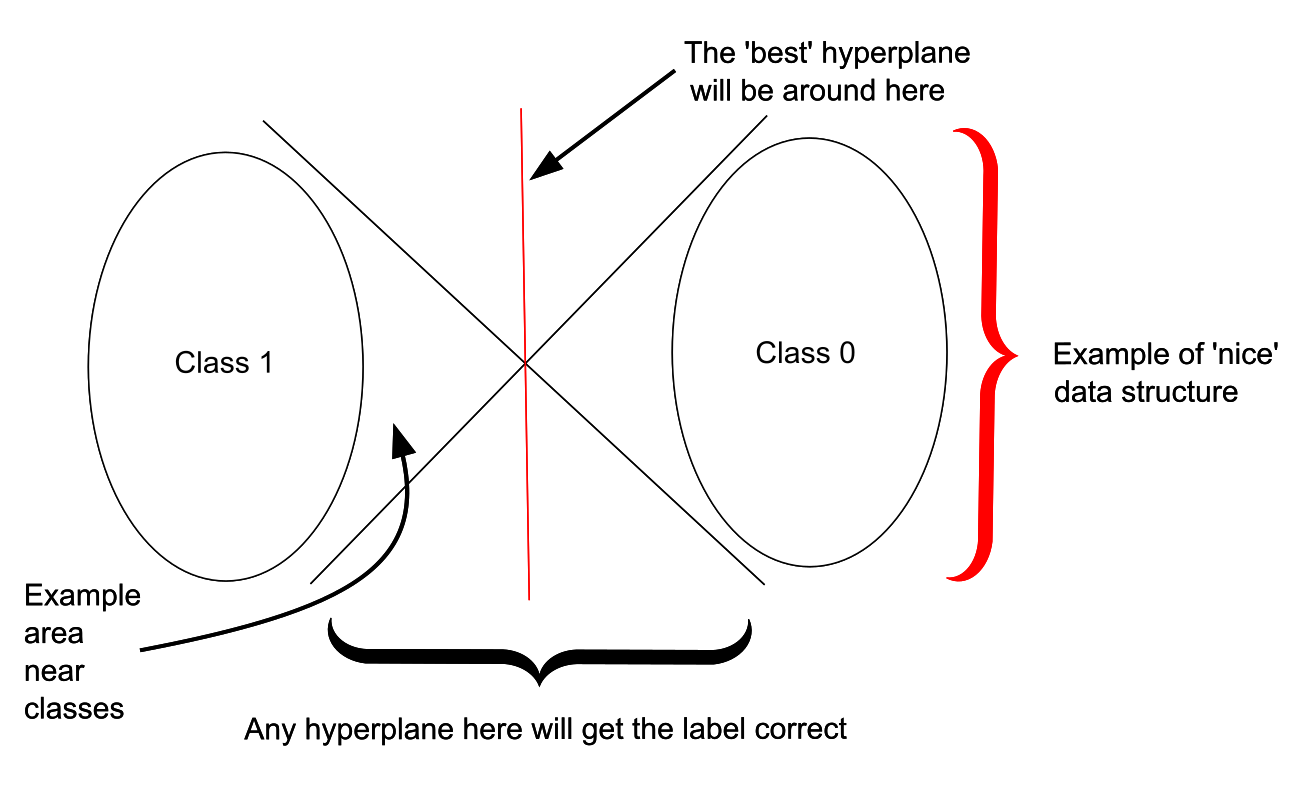
\includegraphics[width=\textwidth]{figs/hyperplanes_good_classes.png}}
\caption{Illustration of well separated classes.} 
\label{fig:good_sep_classes} % labels must come after captions (figures are 'labelable'?)
\end{figure}

Figure \ref{fig:good_sep_classes} shows the desired geometry of the data. In the following two scenarios our reasoning makes the assumption when new examples are fed into the algorithm. They will likely be somewhere around the classes. The ovals indicate the 'clouds' of data that define each class and each line indicates a \gls{decisionboundary} (in a 2D context, this is a line, in a n-d context, these would be \gls{hyperplane}s).  For illustrative purposes, this is a 2D scenario, but it is important to recognise this would generalise up to n-many dimensions.  In this instance, 

\begin{figure}[ht]
\makebox[\textwidth]{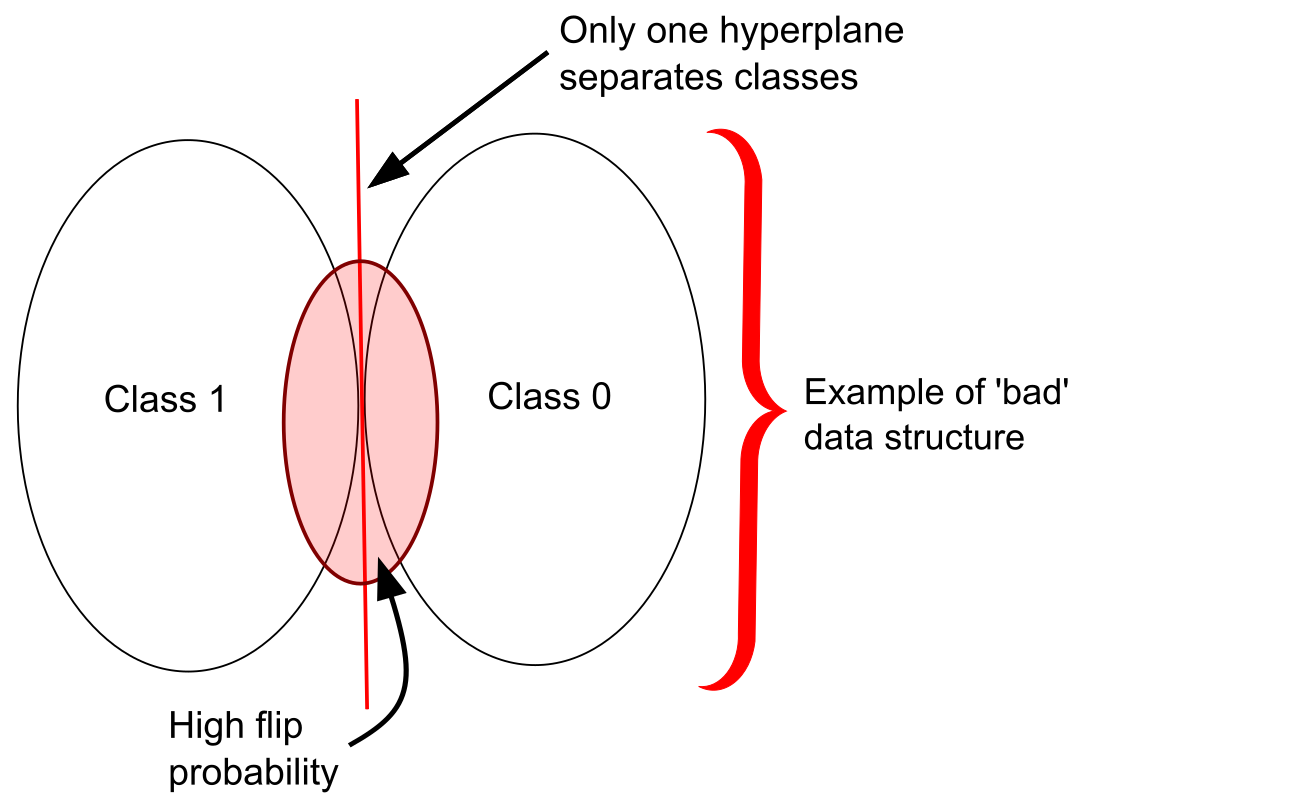
\includegraphics[width=\textwidth]{figs/hyperplanes_poor_classes.png}}
\caption{Illustration of poorly separated classes.}
\label{fig:poor_sep_classes}
\end{figure}

Figure \ref{fig:poor_sep_classes} shows a geometry of the data that would have high flipping probability upon  \gls{rp}. There is only one \gls{hyperplane} that separates the classes. Hence new examples (e.g. out-of-sample data), which are likely to be near this boundary (the area indicated in red) have a high chance of being misclassified. This is an example of a situation where a traditional loss function, such as the \gls{mse}, would have poor \gls{generalisationperformance}, upon learning a \gls{decisionboundary} between these two classes. \bigskip

Calculation of \gls{fp} (compressing the data via  \gls{rp}s) allows for a proxy of how separable the classes are. However, any single \gls{rp} is not likely to find a good representation of the data.

Hence, we wish to find a representation of the data, through many repeated  \gls{rp}s, that shifts the classes away from each other geometrically (i.e. from Figure \ref{fig:poor_sep_classes} to Figure \ref{fig:good_sep_classes}) and hence minimises the \gls{fp} \bigskip

For this, we will need an empirical measure of \gls{fp} and a functioning (trainable) implementation of it in a \gls{cnn}. \bigskip

\gls{fp}